\documentclass[a4paper, 12pt,oneside]{article} 
%\documentclass[a4paper, 12pt,oneside,draft]{article} 
\usepackage{preamble}
%--------------------- ACTUAL FILE ---------------------- %
\begin{document} 
%%%
	\begin{center}
	    \Large
	    \textbf{Coin Data Statistical Study}
	    \vspace{0.4cm}
		\newline
	    \large
		Regression Methods Project \\
	    By Rayan Harfouche \& Tara Fjellman \\
	    \small{Fall 2024}
	\end{center}
	\section{Introduction}
	\lipsum[1]
	\section{Analysis}
	\lipsum[1]
	\begin{table}[htb]
		\centering
		\caption{Model comparison for different models.}
		\label{tab:model-comparison}
		\begin{tabular}{lccc}
		\toprule
		Model & Deviance & AIC & Model DF \\
		\midrule
		1 & 3943.48 & 173.97 & 0 \\
		1+C(person) & 3677.51 & 0.00 & 46 \\
		1+C(person)+C(coin) & 3611.12 & 17.61 & 88 \\
		1+C(person)+C(coin)+C(person):C(coin) & 3460.03 & 108.53 & 209 \\
		\bottomrule
		\end{tabular}
	\end{table}
	\lipsum[1]
	\begin{figure}[htb]
		\centering
		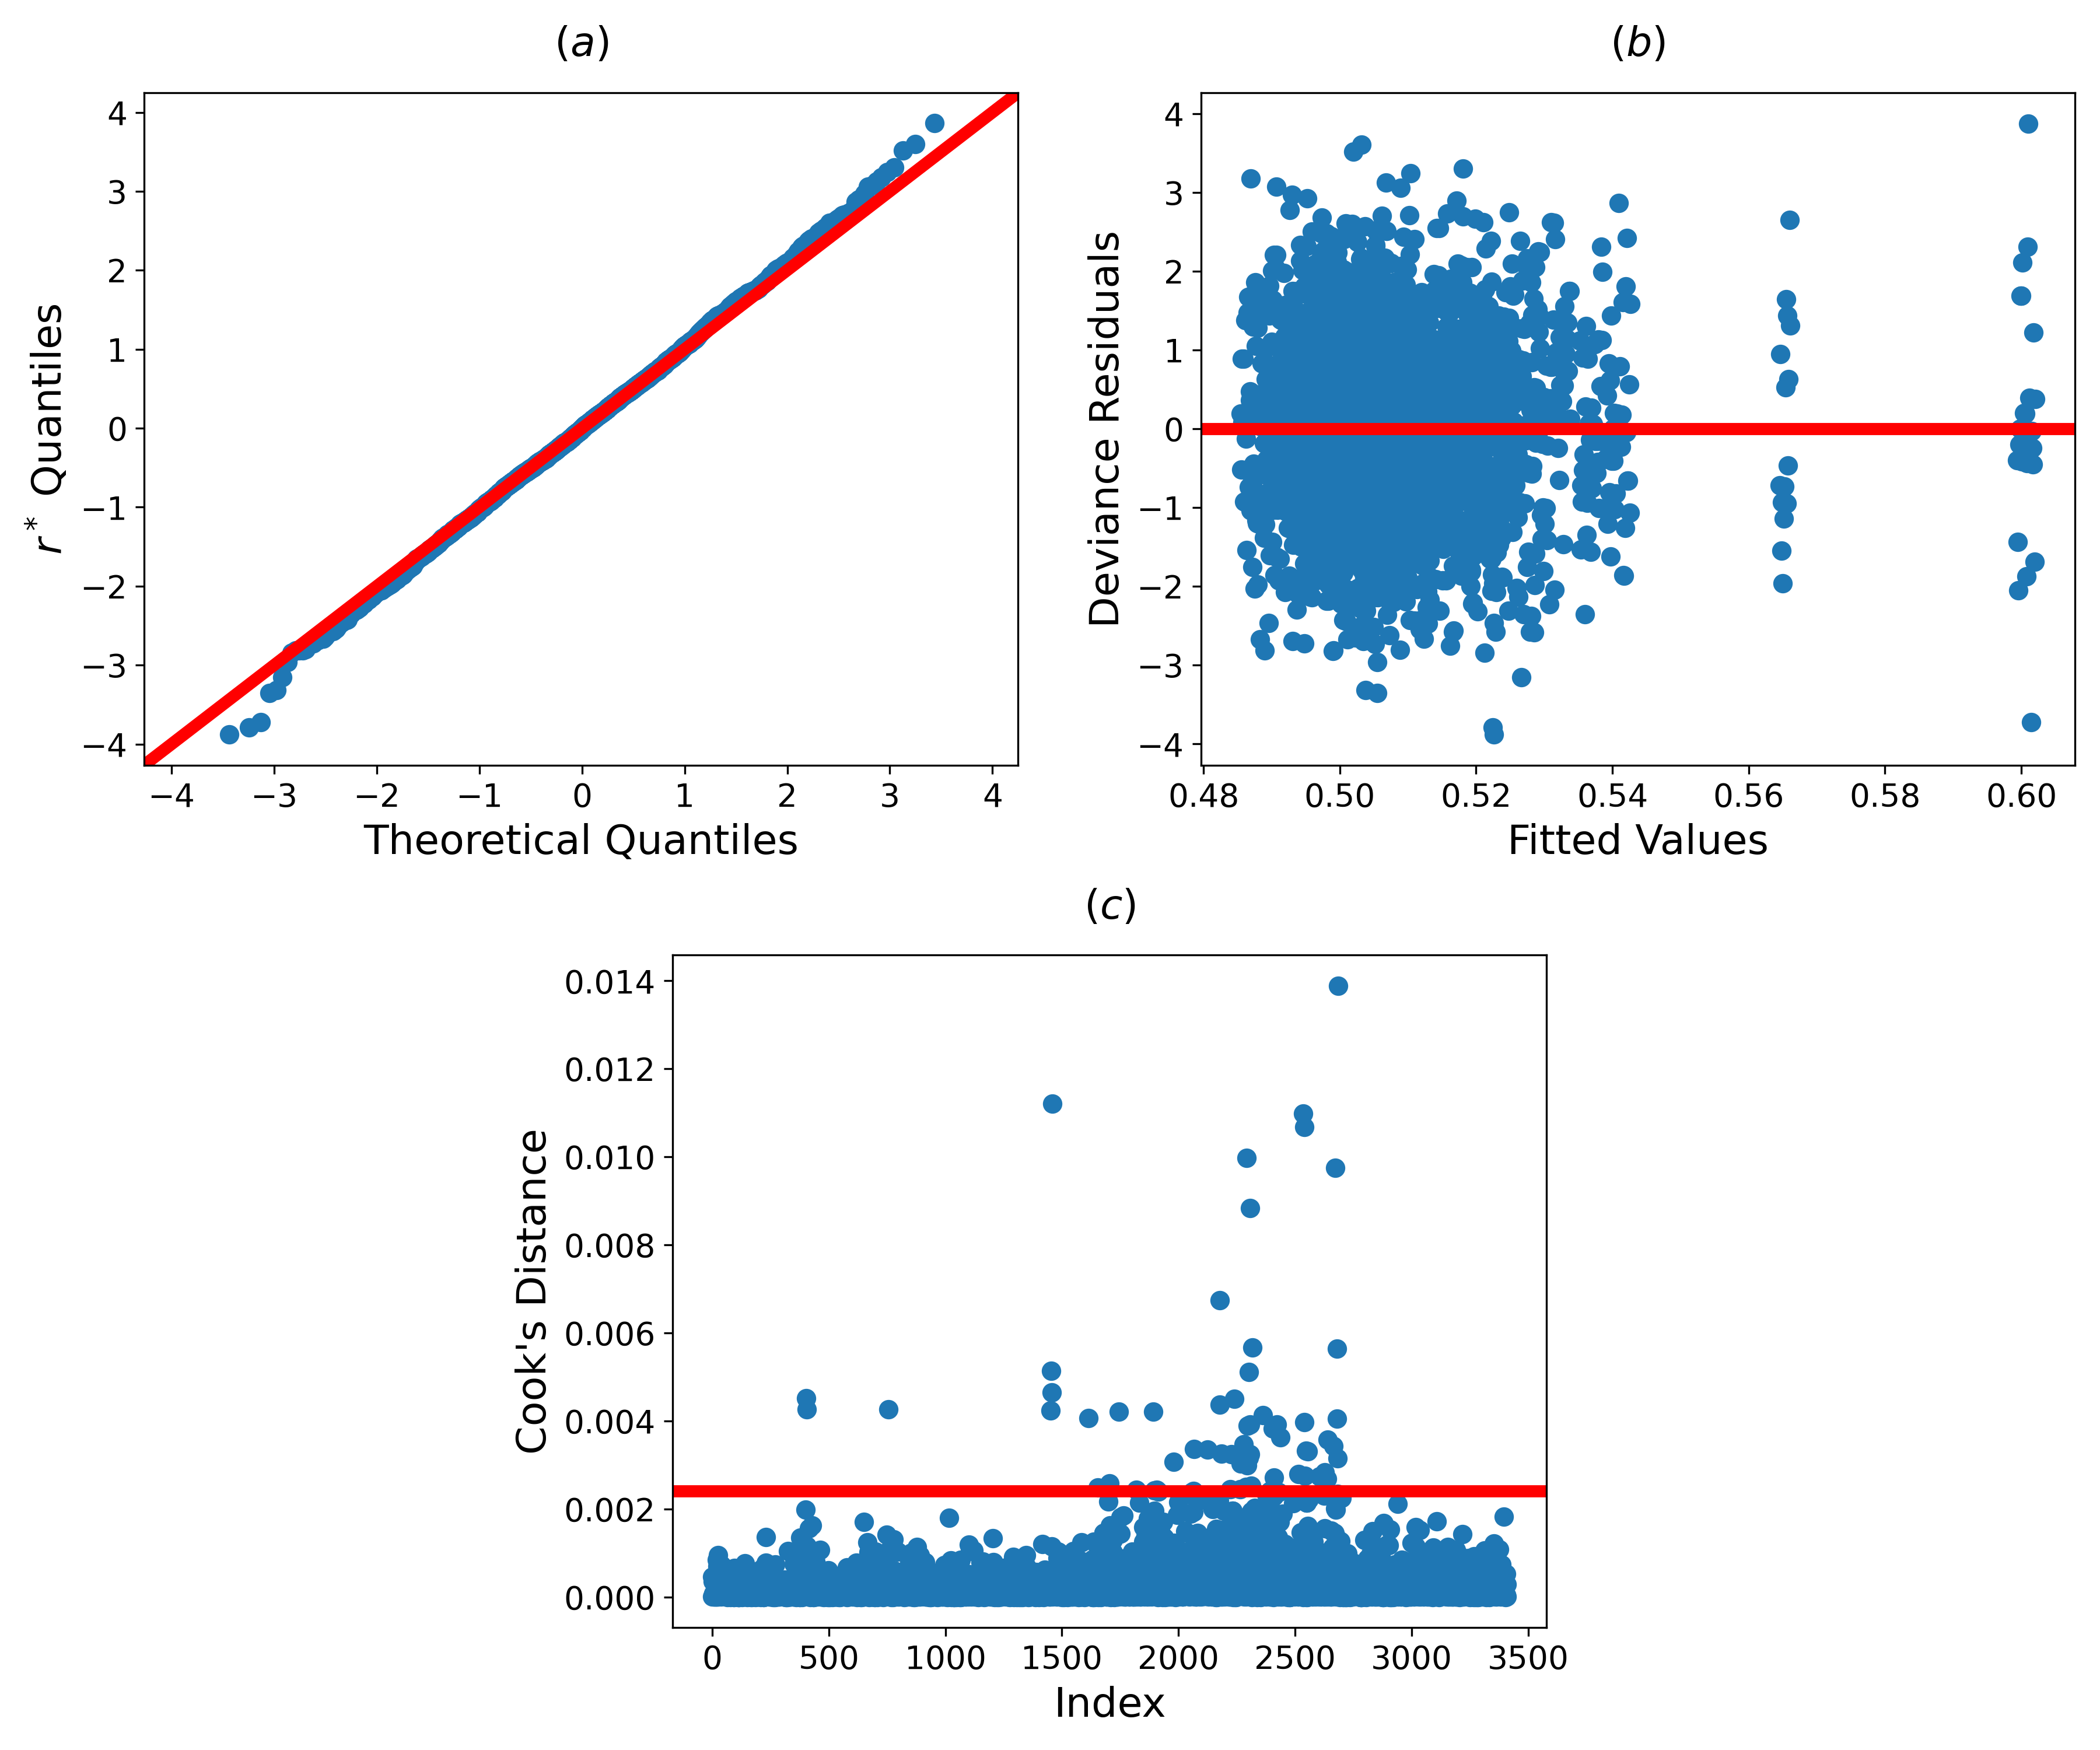
\includegraphics[width=0.85\textwidth]{GLM_diagnostics.png}
		\caption{Diagnostics for the selected GLM model. (a).}
		\label{fig:glm-diagnostic}
	\end{figure}
	\lipsum[1]
	\begin{table}[htb]
		\centering
		\caption{Likelihood ratio tests between models.}
		\label{tab:llr-comparison}
		\begin{tabular}{llc}
		\toprule
		Tested model & Restricted model & $p$-value \\
		\midrule
		1+C(person) & 1 & 0.00e+00 \\
		1+C(person)+C(coin) & 1+C(person) & 9.61e-03 \\
		1+C(person)+C(coin)+C(person):C(coin) & 1+C(person)+C(coin) & 3.32e-02 \\
		\bottomrule
		\end{tabular}
	\end{table}
	\section{Discussion}
	\section{Conclusion}
	\section*{Acknowledgements}
	\section*{References}
	%\appendix
	%	\section{Runtime Estimation}\label{appendix:runtime_estimation}
%%%
\end{document} 